\documentclass[10pt]{beamer}

\usepackage{Theme/BeamerTheme}
\usefonttheme[onlymath]{serif}
\usepackage{hyperref}
\hypersetup{pdfpagemode=FullScreen}
\usepackage{mathrsfs}
\usepackage{amsmath}
\usepackage{bm}
\usepackage{mathtools}
\usepackage{booktabs}
\usepackage{multirow}
\usepackage{ragged2e}
\justifying
\let\raggedright\justifying
\usepackage{tikz}
\usepackage{tkz-euclide}
\usetikzlibrary{decorations.text}
\usetikzlibrary{shadows}
\usetikzlibrary{shapes}
\usetikzlibrary{circuits.logic.CDH}
\usetikzlibrary{arrows.meta}
\usetikzlibrary{decorations.pathmorphing}
\usepackage{pgfplots}
\usepgfplotslibrary{groupplots}
\usepgfplotslibrary{fillbetween}

\tikzset{
    text shadow/.code args={[#1]#2at#3(#4)#5}{
        \pgfkeysalso{/tikz/.cd,#1}%
        \foreach \angle in {0,5,...,359}{
                \node[#1,text=white] at ([shift={(\angle:.8pt)}] #4){#5};
        }
    }
}

\usepackage{tabu}
\usepackage{graphicx}
\usepackage{colortbl}

\usepackage{siunitx}
\ExplSyntaxOn
\cs_new_eq:NN \siunitx_table_collect_begin:Nn \__siunitx_table_collect_begin:Nn
\ExplSyntaxOff

\usepackage{soul}

\DeclareMathSizes{5}{5}{3}{3}

\newcommand{\pgfdefaultlinewidth}{0.75pt}
\newcommand{\risk}{\mathscr{R}}


\begin{document}

% Cover
% \maketitle
\begin{frame}[plain, noframenumbering]\label{Title}
    \vfill
    \centering
    \usebeamerfont{title}\Huge
    Monthly Report\\
    \begin{tikzpicture}\draw[mLightBrown, line width = 1pt] (0, 0) -- (\textwidth, 0);\end{tikzpicture}\vspace{15pt}\\
    \begin{minipage}[m]{3cm}
        \Bold \small Zhang Qi
    \end{minipage}\hspace{-15pt}
    \begin{minipage}[m]{1.5cm}
        \centering
        
\includegraphics[height=0.8cm]{Logos/HUSTLogoWithoutSubline.pdf}
    \end{minipage}
    \begin{minipage}[m]{0.55\textwidth}
        \Normal \scriptsize School of Automation,\\Huazhong University of Science and Technology,\\Wuhan, China.
    \end{minipage}
    \vfill
    \centering
    \usebeamerfont{date}\usebeamercolor[fg]{date}\today
\end{frame}

% Outlines
\begin{frame}[noframenumbering]{Outlines}\label{Outlines}
    \setcounter{tocdepth}{1}
    \tableofcontents % [pausesections]
\end{frame}

% Main Body
\section{Impressions}
% 我们的研究方向是没问题的,现在国内外很多人都在研究这方面内容,周老师从五六年前就开始关注这个方向我打心眼里说周老师还是非常有远见的。
\begin{frame}{We are in the Right Direction.}
    \centering
    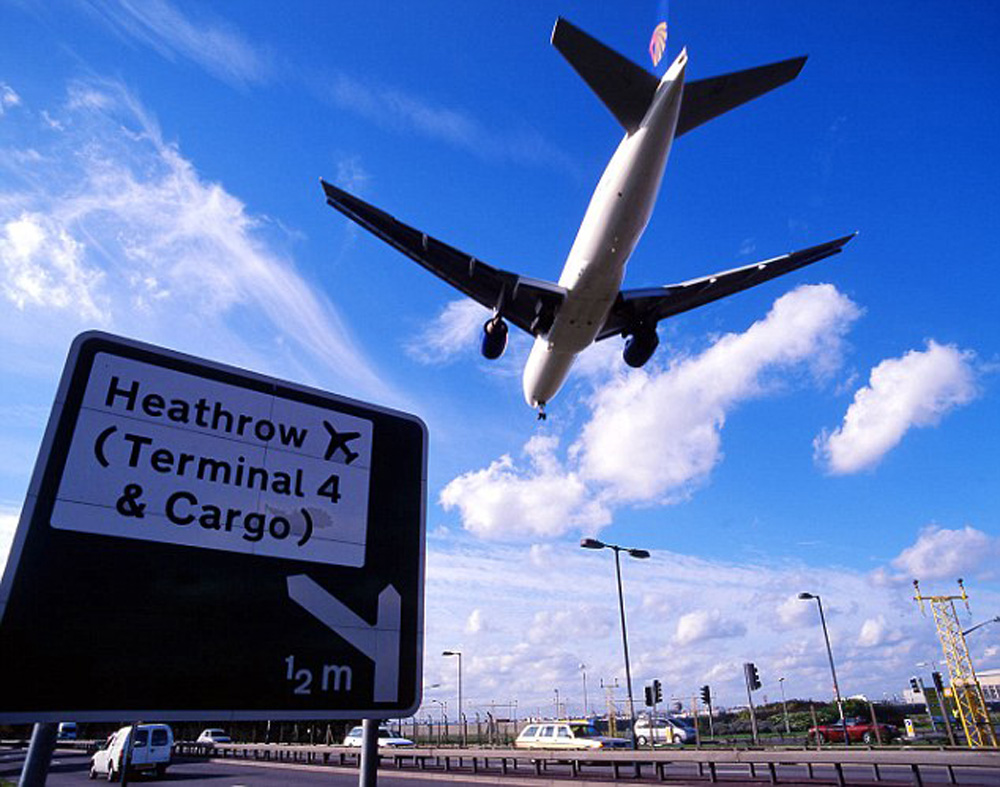
\includegraphics[width=\textwidth, height = 0.9\textheight]{Figures/Heathrow.jpg}
\end{frame}

% 我们的研究进展是处于领先水平的,开会的时候我们发现同行很少做的有我们这么深入的。
\begin{frame}{We are Occupying a Leading Position.}
    \centering
    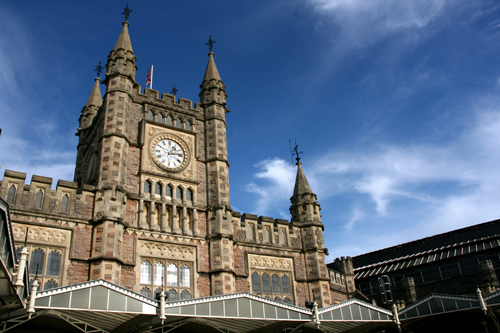
\includegraphics[width=\textwidth, height = 0.9\textheight]{Figures/Bristol.jpg}
\end{frame}

% 交流非常重要,这里的交流指两点,往大了说,是指不同学校、国家之间的学术交流。Scube、Bayes网的仿真工具。往小了说,是指实验室同学之间的交流。
\begin{frame}{Communication is Important.}
    \centering
    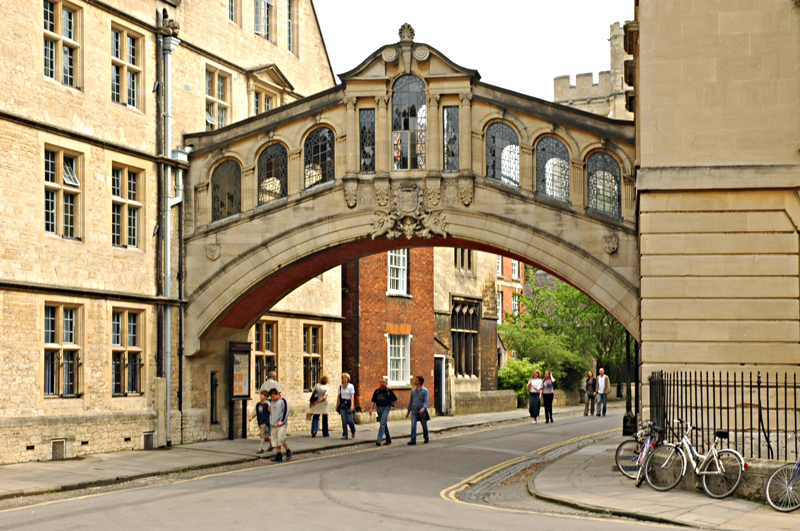
\includegraphics[width=\textwidth, height = 0.9\textheight]{Figures/Oxford.jpg}
\end{frame}

% 实验平台很重要,而且要与实际应用紧密耦合,不能建造空中楼阁。杨老师这方面做的很好,项目都有很强的应用背景,有的甚至有产品,抛开技术含量的问题,这些实物给人的感受远远比一堆论文要来的震撼。
\begin{frame}{Testbed is Important.}
    \centering
    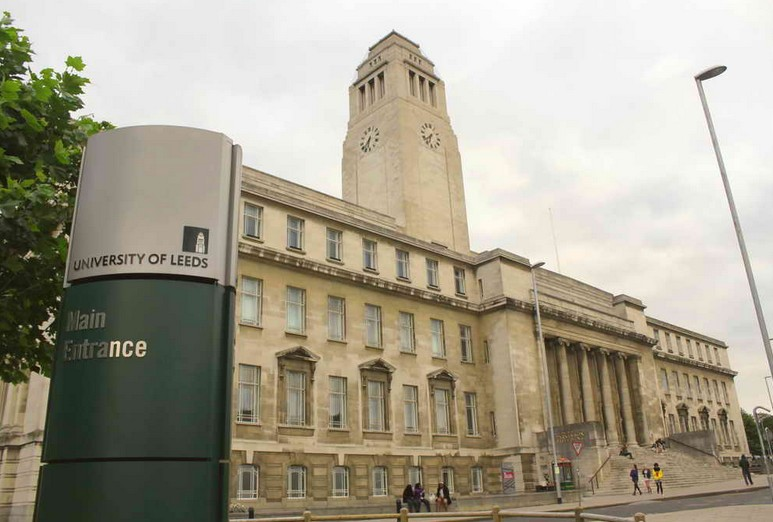
\includegraphics[width=\textwidth, height = 0.9\textheight]{Figures/Leeds.jpg}
\end{frame}

% 英语很重要。一方面是书面表达,写文章的时候很有用,而且不能临阵磨枪,我建议有读博打算的同学趁早学好英语,不要像我,文章因为语言问题耽误很久。另一方面就是听说能力,我前面说过,学术交流是十分重要的,很多学术会议都是英文的,所以英语的口语和听力是十分重要的。周老师基本每年都会带学生出国,我相信,周老师喜欢带英语好的人出国,所以想抓住这个公费出国机会的同学,需要提高英语听说能力。
\begin{frame}{English is Important.}
    \centering
    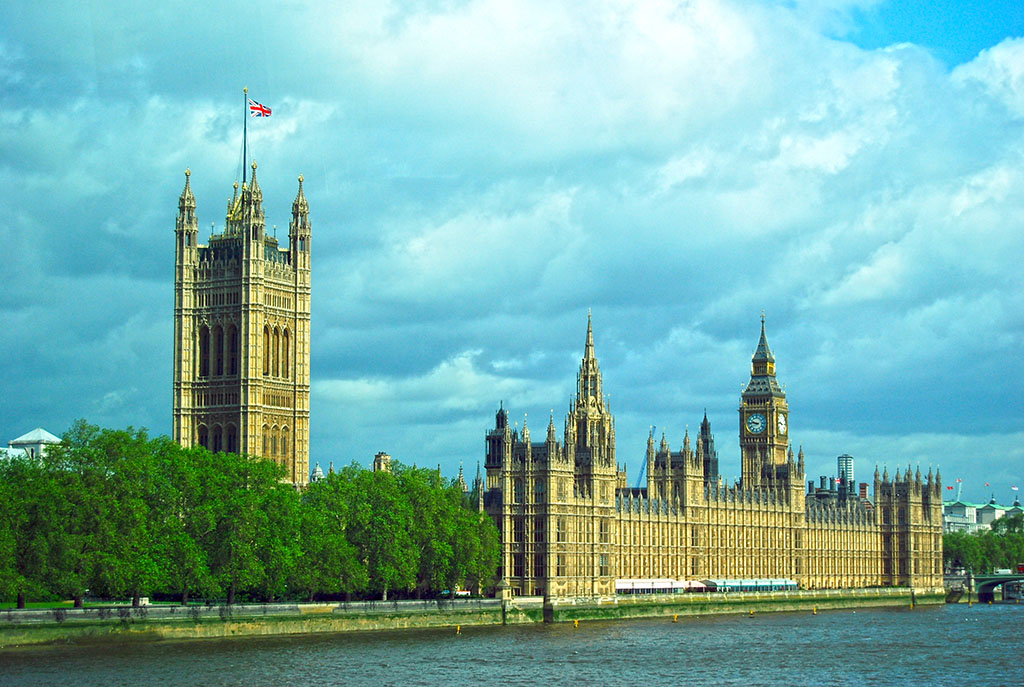
\includegraphics[width=\textwidth, height = 0.9\textheight]{Figures/BigBen.jpg}
\end{frame}

% 我们需要更加自信。开会转了一圈,跟别人交流了很多,同方向的坐到我们这个深度的非常少。
\begin{frame}{We should be More Confident.}
    \centering
    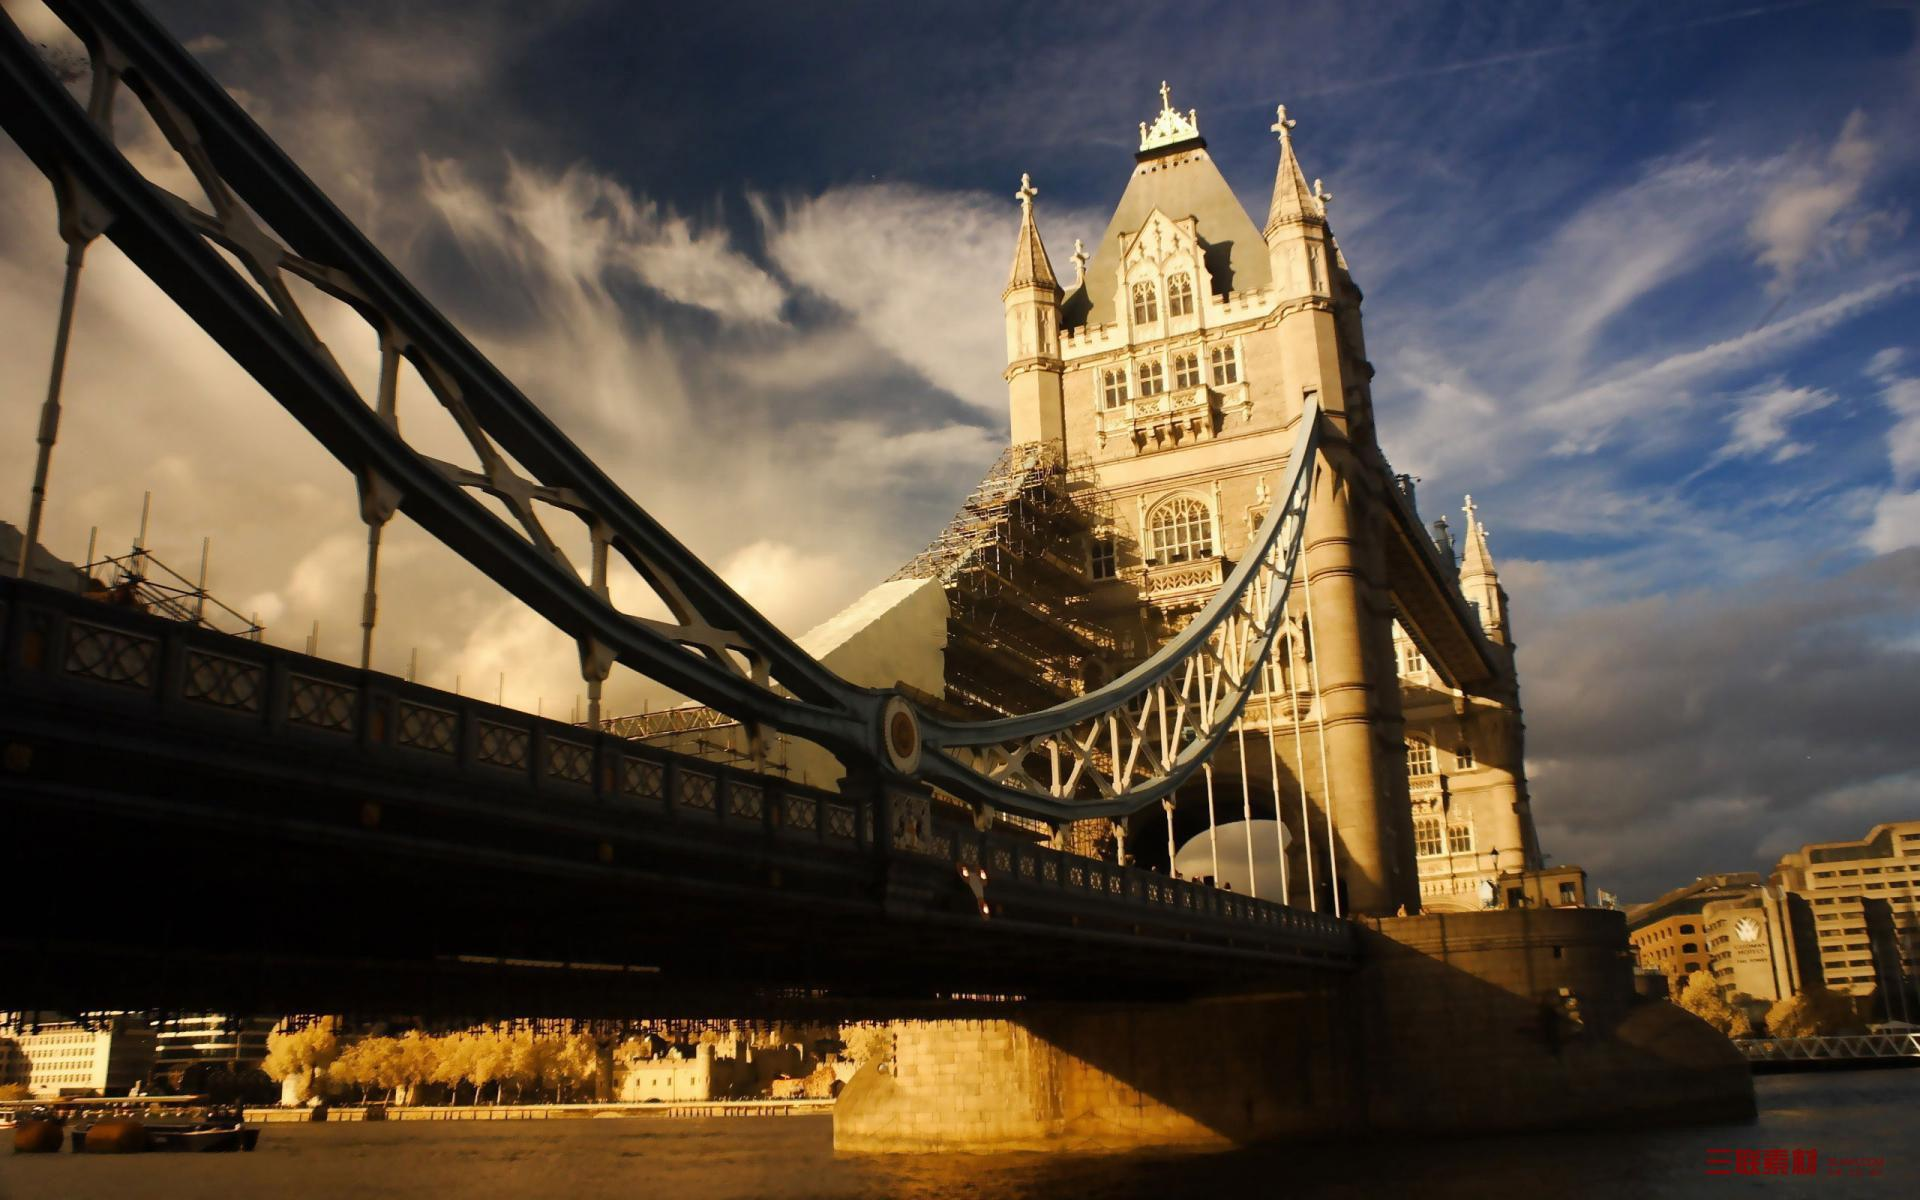
\includegraphics[width=\textwidth, height = 0.9\textheight]{Figures/TowerBridge.jpg}
\end{frame}

% 我们需要更努力的工作。前面我说了,我们的方向没问题,而且处于领先位置,但是现在领先不意味着一直领先。现在国内外做信息安全的人非常非常多,竞争非常激烈,如果我们不及时把我们的研究成果变成论文、专利,那么等别人先发出来就没我们什么事儿了。所以说我们需要更加努力的搞科研。
\begin{frame}{We should Work Harder and Harder.}
    \centering
    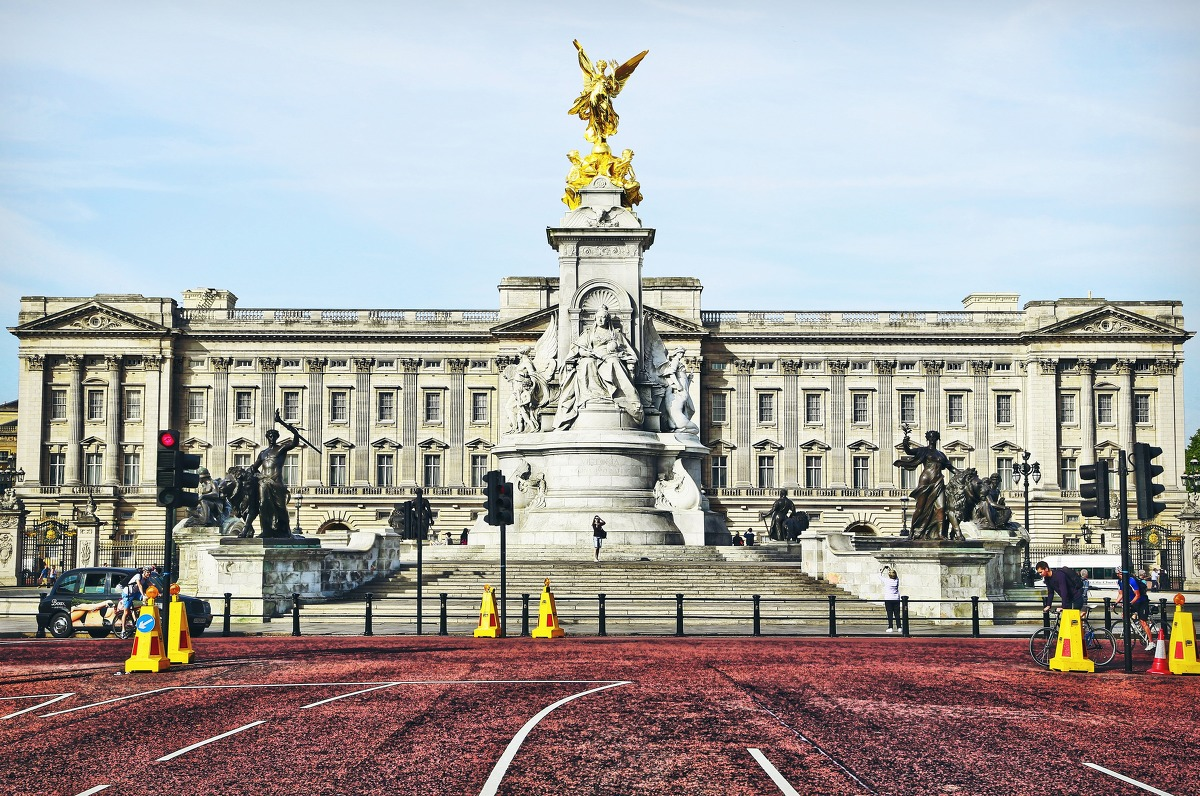
\includegraphics[width=\textwidth, height = 0.9\textheight]{Figures/Buckingham.jpg}
\end{frame}

\section{Task Planning}
\begin{frame}{Task Planning}
    \begin{itemize}
      \item Revise the 1\textsuperscript{st} Paper.
      \item Finish the 2\textsuperscript{nd} Paper.
    \end{itemize}
\end{frame}




\end{document}
